% !TEX root = Master.tex

The next step, after fitting proper models to the marginal distributions of the log-sales aggregated on key category cluster level, is to enter the pairwise modelling of the clusters. Specifically, we are interested in capturing the dependence structures over time which is delineated in the next three subsections (\ref{sssec:kcc_26}, \ref{sssec:kcc_28} and \ref{sssec:kcc_68}).
\\

Recalling the previous Section \ref{ssec:kcc_margins}, the residuals from the fitting methods are depicted in \autoref{fig:res_gamlss_over_time} for each time-point. In a second step after the marginal modelling in Section \ref{ssec:kcc_margins}, the residuals are used in a pairwise fashion to estimate the dependence structures with the help of conditional copulas (see Section \ref{ssec:conditional_copulas}).\footnote{Currently, the \textit{GJRM} package supports trivariate copula functionalities for binary responses only \citep{marragjrm}.}
\\

\begin{figure}[H]
\centering
  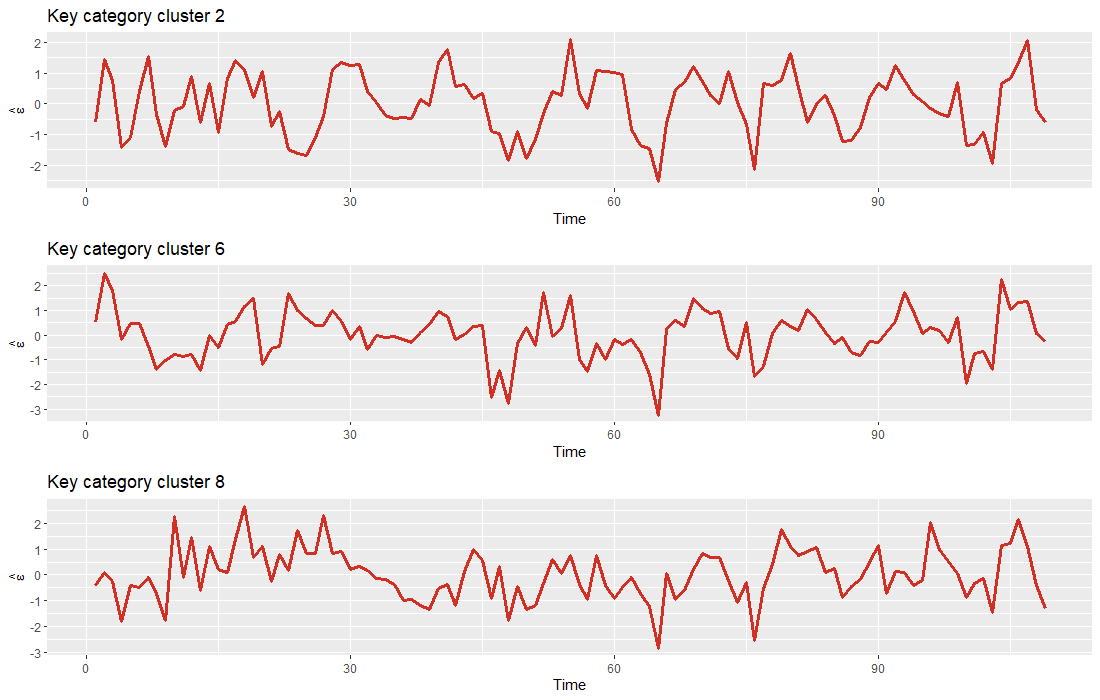
\includegraphics[width=0.95\linewidth]{figures/res_gamlss_over_time.png}
  \caption{Estimated residuals of GAMLSS fits for the three key category clusters}
  \label{fig:res_gamlss_over_time}
\end{figure}










In the previous section (\ref{ssec:kcc_margins}), the model fits resulted in quantile residuals that we were able to approximate parametrically by normal distributions. \\
Moreover, the only distributions that are at the disposal of both the \textit{gamlss} package \citep{rigby2005generalized} and the \textit{GJRM} package\footnote{Elaboration on this in the following subsections.} \citep{marragjrm} are the normal and the logistic distributions. The \ac{AIC} values of these distributions are close, indicating that both are good fits (see \nameref{sec:appendix}, R output \ref{output:gamlss_distributions_aic}). Thus, in the following the normal distribution is chosen as response family for all three residual sets.


